\section{Brownie Point Nominations}

\begin{frame}{Integral Attack on Round Reduced PRINCE}
\begin{enumerate}
    \item We know that integral cryptanalysis works for block ciphers with substitution-permutation network and PRINCE falls in this category.
    \item 3.5 round integral distinguisher
    \item Notion of Active nibble
    \item 4-round attack as well as 5-round attack
\end{enumerate}

\end{frame}

\begin{frame}{Integral Attack on Round Reduced PRINCE}
\textbf{The 3.5 round distinguisher}
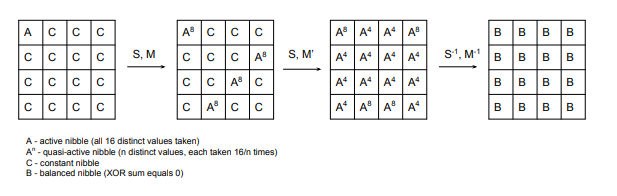
\includegraphics[scale=0.5]{Presentation/dfcdfsd.png}
\begin{center}
How $M'$ affects an active nibble?
\end{center}
\end{frame}

\begin{frame}{4-round Integral Attack} 
\textbf{Recovery of $k'_0\oplus k_1$}
\begin{itemize}
    \item Take $2^4$ plaintexts with one active nibble
    \item Make a guess for nible of $k'_0 \oplus k_1$ and decrypt partially through last Sbox
    \item Check if nibble is balanced or not
    \item Repeat this for 16 nibbles
    \item To remove false positives use 5 sets
\end{itemize}

\end{frame}
\begin{frame}{4-round Integral Attack}
\textbf{Recovery of $k_1$}
\begin{itemize}
    \item Start with 5 sets of $2^4$ plaintexts with 4 active nibbles and peel of last round using $k'_0\oplus k_1$
    \item Notion of 2.5 round distinguisher
    \item Invert linear layer and partially decrypt through 1 sbox
    \item Check if nibble is balanced
    \item Data complexity is 2x5x$2^4 \approx 2^7$, Time complexity is 16x2x5x$2^4 \approx 2^{11}$
\end{itemize}
We have implemented the attack in python.
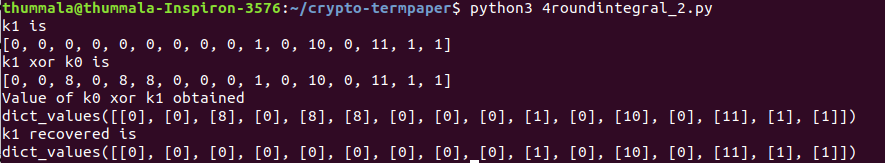
\includegraphics[scale=0.29]{Presentation/dssdfsdf.png}
\end{frame}
\begin{frame}{5-round Integral Attack}
    This is an extension of 4-round attack. The method is as follows:
    \begin{itemize}
        \item Take 6 sets of $2^4$ plaintexts with 1 active nibble each.
        \item Balanced property gets destroyed after 4th round and 5th round sbox.
        \item Hence make a guess of a column of $k'_0 \oplus k_1$, partially decrypt through last Sbox and M-layer
        \item Guess a particular nibble of $k_1$ and partially decrypt through 1 more sbox and check whether nibble is balanced to obtain $k'_0 \oplus k_1$
        \item Peel of last layer and guess $k_1$ nibble by nibble as in 4-round attack except we only need to decrypt through one sbox.
    \end{itemize}
\end{frame}